\chapter{Аналитический раздел}

В данном разделе приводятся анализ предметной области и этапы очистки и предварительной обработки текста, также рассматривается обзор методов извлечения признаков из текста. Также анализируются основные методы классификации текстов и проведено сравнение методов классификации текстов по преимуществам и недостаткам. Также в этом разделе представляется формализованная постановка задачи в виде IDEF0-диаграммы.

\section{Анализ предметной области}
\subsection{Задача классификации текстов}
Классификация текста —-- это процесс присвоения предопределенной категории или метки предложениям, абзацам, текстовым отчетам или неструктурированного текста.

За последние несколько десятилетий проблемы классификации текста широко изучались и решались во многих практических приложениях. Многие исследователи теперь заинтересованы в разработке приложений, использующих преимущества методов классификации текста, особенно в связи с недавними достижениями в области обработки естественного языка.

Некоторые задачи классификации текста в реальном \cite{task}:
\begin{enumerate}
    \item анализ настроений --- задача понимания аффективных состояний и субъективной информации, содержащейся в фрагменте текста;
    \item маркировка тем --- задача распознавания одной или нескольких тем фрагмента текста (т. е. его тем);
    \item классификация новостей --- задача присвоения новостям категорий;
    \item ответ на вопрос --- задача выбора ответа на вопрос, выбора из потенциальных предложений - кандидатов (обычно извлекаемых из контекстного документа);
    \item вывод на естественном языке --- задача определения того, влекут ли два предложения друг друга (классификация, происходит ли следование в одном из двух направлений или ни в одном из них);
    \item распознавание именованных объектов --- задача поиска именованных объектов в неструктурированном тексте и маркировка их заранее определенными категориями;
    \item синтаксический анализ --- серия задач, связанных с прогнозированием морфо - синтаксических свойств слов.
\end{enumerate}
\subsection{Процесс классификации текста}

Большинство процессов классификации текста, обычно, состоят из следующих трёх шагов: предобработка текста, извлечение признаков и классификации текста с помощью некоторого алгоритма. 

Ниже, на рисунке \ref{img:system}, представлены этапы процесса классификации текста.\newline
\captionsetup{justification=centering,singlelinecheck=off}
\begin{figure}[h!]
	\centering
		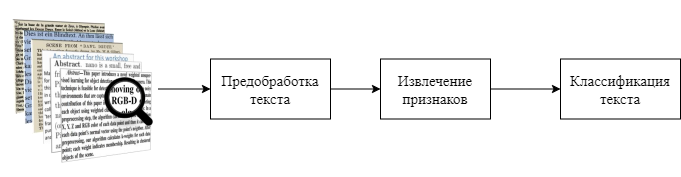
\includegraphics[,scale=0.7]{./img/system.png}
		\caption{Этапы процесса классификации текста.}  
		\label{img:system}
\end{figure}


Система классификации текстов содержит четыре различных уровня области применения, которые можно применять.
\begin{enumerate}
    \item Уровень документа. На этом уровне документа алгоритм получает соответствующие категории полного документа.
    \item Уровень абзаца. На этом уровне абзаца алгоритм получает соответствующие категории одного абзаца (части документа).
    \item Уровень предложения. На этом уровне предложения получают соответствующие категории одного предложения (части абзаца).
    \item Уровень подпредложения. На этом уровне подпредложения алгоритм получает соответствующие категории подвыражений внутри предложения.
\end{enumerate}
\section{Предобработка текста}
\subsection{Необходимость предобработки текста}

Входные данные для задач на естественном языке состоят из необработанного неструктурированного текста. Текстовая информация, в отличие от других типов данных, таких как изображения или временные ряды, не обладает числовым представлением, поэтому перед подачей ее в какой-либо классификатор она должна быть спроецирована в соответствующее пространство признаков. Поэтому процедуры предварительной обработки имеют особое значение, поскольку без них не существует основы ни для процедур выделения признаков, ни для алгоритмов классификации.

\subsection{Очистка и предобработка текста}
\textbf{Токенизация} --- самая базовая операция предварительной обработки, которую необходимо применить к тексту. Этот процесс определяет уровень детализации анализа текстовых данных и в целом может быть описан как процесс предварительной обработки, целью которого является разделение текстового потока на слова, фразы, символы или другие значимые элементы, называемые токенами. Разделение основано на правилах и может быть простым, как разделение пробелами или знаками препинания.

Например, предложение:

After eating, I decided to start working.

В данном случае токены следующие:

\{“After”, “eating”, “I”, “decided”, “to”, “start”, “working”\}.

\textbf{Стоп-слова} (текстовые шумы) —-- это неинформативные слова, которые встречаются в большом количестве, но не имеют семантического значения. Например, слова ``и'', ``в'', ``только'' не несут никакой ценности и только добавляют шум в данные. Множество токенов, полученный после процесса токенизации, может содержать множество ненужных или бессмысленных элементов. Удаление стоп-слов необходимо, поскольку это уменьшит количество различных элементов в пространстве признаков. 

Обычно тексты содержат разные грамматические формы одного и того же слова, а также могут встречаться однокоренные слова. Лемматизация и стемминг преследуют цель привести все встречающиеся словоформы к одной, нормальной словарной форме. 

\textbf{Стемминг} –-- это грубый эвристический процесс, который отрезает ``лишнее'' от корня слов, часто это приводит к потере словообразовательных суффиксов. 

\textbf{Лемматизация} –-- это более тонкий процесс, который использует словарь и морфологический анализ, чтобы в итоге привести слово к его канонической форме –-- лемме. 

Отличие в том, что стеммер (конкретная реализация алгоритма стемминга) действует без учёта контекста и, соответственно, не делает разницы между словами, которые имеют разный смысл в зависимости от части речи. Однако у стеммеров есть своё преимущество –-- они работают быстрее.
\section{Извлечения признаков}
\subsection{Модель Bag of Words}
\textbf{Модель Bag of Words} (модель BoW)\cite{phan1} —-- это уменьшенное и упрощенное представление текстового документа из выбранных частей текста на основе определенных критериев, таких как частота слов.

При всей простоте реализации данный подход имеет ряд недостатков:

\begin{itemize}[label = ---]
    \item для больших наборов текстов размерность словаря, а, следовательно, и размерность вектора, представляющего текст, может исчисляться сотнями тысяч, а иногда и миллионами;
    \item не учитывается контекст слова в документе.
\end{itemize}
\subsection{Метод Word2Vec}
\textbf{Word2Vec} (Word to Vector)\cite{phan1} —-- это метод, используемый для преобразования слов в векторы, тем самым фиксируя их значение, семантическое сходство и взаимосвязь с окружающим текстом. Этот метод помогает компьютерам изучать контекст и значение выражений и ключевых слов из больших текстовых коллекций, таких как новостные статьи и книги.

Основная идея Word2Vec состоит в том, чтобы представить каждое слово как многомерный вектор, где положение вектора в этом многомерном пространстве отражает значение слова.

Word2Vec использует модель мелкой нейронной сети для изучения значения слов из большого массива текстов. В отличие от глубоких нейронных сетей, которые имеют несколько скрытых слоев, мелкие нейронные сети имеют только один или два скрытых слоя между входом и выходом. Это делает обработку быстрой и прозрачной. Неглубокая нейронная сеть Word2Vec может быстро распознавать семантические сходства и идентифицировать слова-синонимы, что делает ее быстрее глубоких нейронных сетей.
\subsection{Алгоритм GloVe}
\textbf{GloVe} (Global Vector)\cite{phan1} --- алгоритм обучения без учителя  для получения векторных представлений слов. Обучение проводится на основе агрегированной глобальной статистики частоты совпадения слов из корпуса, и полученные представления демонстрируют интересные линейные подструктуры векторного пространства слов.  

Преимущества GloVe:
\begin{itemize}[label = ---]
    \item простая архитектура без нейронной сети;
    \item модель быстрая, и этого может быть достаточно для простых приложений;
    \item GloVe улучшает Word2Vec. Она добавляет частоту встречаемости слов и опережает Word2Vec в большинстве приложений;
    \item осмысленные эмбеддинги.
\end{itemize}

Недостатки алгоритма:
\begin{itemize}[label = ---]
    \item хотя матрица совместной встречаемости предоставляет глобальную информацию, GloVe остаётся обученной на уровне слов и даёт немного данных о предложении и контексте, в котором слово используется;
    \item плохо обрабатывает неизвестные и редкие слова.
\end{itemize}
\subsection{FastText}
\textbf{FastText}\cite{phan1} —-- это созданная в Facebook библиотека, содержащая предобученные готовые векторные представления слов и классификатор, то есть алгоритм машинного обучения разбивающий тексты на классы.

К основной модели Word2Vec добавлена модель символьных n-грамм. Каждое слово представляется композицией нескольких последовательностей символов определённой длины. Например, слово they в зависимости от гиперпараметров, может состоять из “th”, “he”, “ey”, “the”, “hey”. По сути, вектор слова – это сумма всех его n-грамм.

Результаты работы классификатора хорошо подходят для слов с небольшой частотой встречаемости, так как они разделяются на n-граммы. В отличие от Word2Vec и Glove, модель способна генерировать эмбеддинги для неизвестных слов.
\subsection{TF-IDF}
\textbf{TF-IDF} (англ. term frequency-inverse document frequency) --- статистическая мера, используемая для
оценки важности слова в контексте документа. Большой вес в TF-IDF получают слова с высокой частотой в пределах конкретного документа и с низкой частотой употребления в других документах. Вычисление вес в TF-IDF состоит из трех этапов. Первым этапом выполняется подсчет доли вхождений каждого слова (TF) по формуле (\ref{eq:TF}).
\begin{equation}\label{eq:TF}
	TF(word) = \frac{W(word)}{A},
\end{equation}
где W(word) --- количество вхождений слова word в документ, A --- количество всех слов в документе.

Вторым этапом выполняется измерение того, насколько важно это слово (IDF) по формуле (\ref{eq:IDF}).
\begin{equation}\label{eq:IDF}
    IDF(word) = \log\frac{D}{DW(word)} ,
\end{equation}
где D --- общее количество документов, DW(word) --- количество документов, которые содержат слово word.

И третий этап совмещает первые две оценки.
\begin{equation}\label{eq:TFIDF}
    TF-IDF(word) = TF(word) \cdot IDF(word).
\end{equation}

TF-IDF предоставляет несколько ключевых преимуществ.
\begin{enumerate}
    \item Учет важности слов: TF-IDF учитывает как частоту слова в документе, так и его общую редкость по всей коллекции. Таким образом, он помогает выделять ключевые слова, которые часто встречаются в данном документе, но не слишком распространены в остальных.
    \item Устранение шума: Слова, которые встречаются в большинстве документов (стоп-слова), имеют низкий IDF и, следовательно, низкий общий вес TF-IDF. Это позволяет устранить шум и фокусироваться на более важных словах.
\end{enumerate}

\section{Основные методы классификации текстов}
\subsection{Логистическая регрессия}
При совместном обучении с учителями логистическая регрессия --- это выбор наилучших параметров для маркировки для получения эффективных результатов классификации. Логистическая регрессия похожа на линейную регрессию, поскольку нужно найти значения коэффициентов входных переменных. Разница декоммутируется в том, что выходные значения преобразуются с использованием нелинейных или логистических функций.

В зависимости от того, как вы обучаете свою модель, можно использовать оценки логистической регрессии для отображения вероятностей выборок, относящихся к классу 0 или 1. Это полезно, когда нужно повысить точность прогнозирования.

Как и в случае с линейной регрессией, логистическая регрессия лучше справляется со своей задачей, если вы удаляете ненужные аналогичные переменные. Модели логистической регрессии быстро усваиваются и подходят для задач двоичной классификации.

\subsection{Наивный байесовский классификатор}

Это вероятностный классификатор, обычно используемый в машинном обучении, но также может использоваться в качестве статистического метода. В основном он используется для предварительной обработки данных, поскольку его легко вычислить. Для прогнозирования целевого класса используются байесовское рассуждение и вероятностный вывод. Поскольку атрибуты играют важную роль в классификации, производительность может быть улучшена путем присвоения атрибутам различных весовых коэффициентов \cite{11}.

Производительность наивного байесовского классификатора зависит от точности оценки условной вероятности. Без достаточного количества обучающих данных трудно точно оценить эти условия. Поэтому для оценки условных вероятностей используются некоторые методы метаэвристики, такие как генетические алгоритмы и дифференциальная эволюция. В некоторых случаях преимущества этого классификатора ставятся под сомнение из-за условного предположения о независимости между атрибутами, которые влияют на эффективность классификации \cite{11}. Используются различные методы мета-обучения для повышения производительности, включая расширение структуры, выбор атрибутов, преобразование частоты, взвешивание атрибутов, взвешивание экземпляров и локальное обучение. Таким образом, наивный байесовский классификатор прост в реализации и в то же время эффективен с точки зрения надежности. Эти особенности делают классификаторы подходящими для решения задач обработки естественного языка.

\subsection{Метод опорных векторов}
Метод опорных векторов (англ. support vector machine, SVM) --- один из наиболее популярных методов обучения, который применяется для решения задач классификации, регрессии и обнаружения выбросов. Основная идея метода заключается в построении гиперплоскости, разделяющей объекты выборки оптимальным способом. В двумерном пространстве эту оптимальную гиперплоскость можно представить как линию, разделяющую пространство на две части: где одна часть пространства содержит точки данных, которые принадлежат одному классу, а другая часть пространства содержит точки данных, принадлежащие другому класс. Концепция линий, действующих как классификатор, верна только в том случае, если точки данных линейно разделимы. SVM также можно использовать для поиска оптимальной кривой, которая может использоваться для классификации точек данных, которые нельзя разделить линейно.


Преимущества метода:
\begin{itemize}[label = ---]
	\item хорошо работает с пространством признаков большего размера;
	\item метод находит разделяющую полосу максимальной ширины, позволяет в дальнейшем осуществлять более уверенную классификацию;
    \item метод использует подмножество обучающих точек в функции принятия решений (называемых опорными векторами), поэтому это также эффективно с точки зрения памяти.
\end{itemize}

Недостатки метода:
\begin{itemize}[label = ---]
	\item долгое время обучения (для больших наборов данных);
	\item неустойчивость к шуму: выбросы в исходных данных становятся опорными объектами-нарушителями и напрямую влияют на построение разделяющей гиперплоскости.
\end{itemize}

\subsection{Decision Tree and Random Forest}
Деревья решений (англ. Decision Tree) являются одними из самых ранних и популярных классификаторов\cite{45}. Структура этого метода представляет собой иерархическую декомпозицию пространства данных\cite{7}. Основная идея заключается в создании дерева на основе атрибута для категоризированных точек данных, но основная задача дерева решений заключается в том, какой атрибут или функция может находиться на родительском уровне, а какой должен быть на дочернем уровне\cite{161}.

Деревья решений работает в определенной последовательности, чтобы проверить соответствие решения определенному пороговому значению среди доступных значений. Тестирование выполняется в соответствии с определенными логическими правилами, аналогичными весам нейронной сети. На этапе роста дерева обучающий набор разбивается на части, а на этапе обрезки его данные суммируются. Деревья, основанные на ансамбле, используют методы расширения возможностей и упаковки для объединения нескольких классификаторов, которые используют разные правила принятия решений для разных наборов данных \cite{8}. Эти ансамбли показали выдающуюся производительность по сравнению с традиционными деревьями решений, но вычислительные затраты увеличиваются по мере добавления входных запросов \cite{8}.

Дерева решений обладают низкой эффективностью при обработке многомерных данных. Для решения этой проблемы предлагаются кластерные деревья. Инкрементные деревья принятия решений лучше всего подходят для потоков данных, поскольку они обладают способностью стабилизироваться в соответствии с накапливающимися данными. Они использует несколько атрибутов для обучаемых функций.

Ниже, на рисунке \ref{tree}, представлен принцип работы метода деревьев решений.
\captionsetup{justification=centering,singlelinecheck=off}
\begin{figure}[h!]
	\centering
		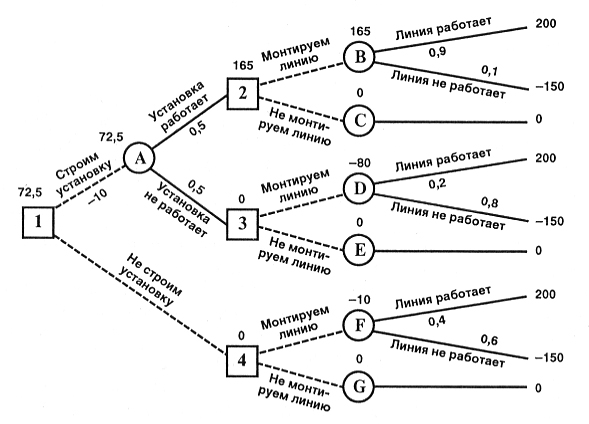
\includegraphics[,scale=1.3]{./img/decision_tree.png}
		\caption{Принцип работы метода деревьев решений}  
		\label{tree}
\end{figure}

Метод случайных лесов (Random Forest) --— это метод обучения для классификации текста. Случайные леса представляют собой наборы деревьев решений, обученных с использованием случайных подмножеств признаков, которые достигли гораздо более высокой производительности и чаще используются на практике. Этот метод очень быстро обучается работе с наборами текстовых данных по сравнению с другими методами, такими как глубокое обучение, но довольно медленным для создания прогнозов после обучения\cite{172}. Таким образом, чтобы добиться более быстрой структуры, количество деревьев в лесу необходимо уменьшить, поскольку большее количество деревьев в лесу увеличивает временную сложность на этапе прогнозирования.

\subsection{Метод K-ближайших соседей}
Метод K-ближайших соседей (англ. K-nearest neighbors, KNN) –-- это простой алгоритм машинного обучения с учителем, который можно использовать для решения задач классификации и регрессии.

Алгоритм K-NN сохраняет все доступные данные и классифицирует новую точку данных на основе сходства. Это означает, что когда появляются новые данные, их можно легко классифицировать по категории наборов с помощью алгоритма K-NN.

Согласно принципу алгоритма KNN, структура классификатора включает в себя 4 параметра: данные для классификации, набор выборочных данных, набор выборочных меток и значение K. Затем вычислить расстояние между новыми данными и выборочными данными, упорядочить расстояния от наименьшего к наибольшему, возьмите первые K ближайших данных. Наиболее часто встречающаяся метка может быть идентифицирована как новая метка данных путем определения количества вхождений каждого введенного типа данных в К первых точках.

Ниже, на рисунке \ref{knn}, представлен принцип работы метода K-ближайших соседей.
\captionsetup{justification=centering,singlelinecheck=off}
\begin{figure}[h!]
	\centering
		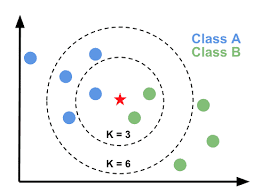
\includegraphics[,scale=1.0]{./img/knn.png}
		\caption{Принцип работы метода K-ближайших соседей}  
		\label{knn}
\end{figure}

Преимущества метода.
\begin{enumerate}
	\item Алгоритм прост и легко реализуем.
	\item Нет необходимости строить модель, настраивать несколько параметров или делать дополнительные допущения.
	\item Алгоритм универсален. Его можно использовать для обоих типов задач: классификации и регрессии.	
\end{enumerate}

Недостатки метода.
\begin{enumerate}
	\item Из аргумента выше следуют большие вычислительные затраты во время выполнения.
	\item Алгоритм работает медленнее при увеличении объема выборки.
	\item Всегда нужно определять оптимальное значение k.
\end{enumerate}

\subsection{Искусственные нейронные сети}
Искусственные нейронные сети (англ. Artificial Neural Network, ANN) имитируют работу человеческого мозга при принятии решений. Они работают, обучаются и развиваются с минимальным вмешательством человека или без него. Для классификации данных был предложен конкурентный алгоритм коэволюции, основанный на модели нейронной сети. Радиальные базовые функции являются компонентом ANN, поскольку они используют более быстрые алгоритмы обучения. Эта функция имеет компактную сетевую архитектуру, повышающую точность классификации. Кроме того, развив октябрьские алгоритмы, как правило, хорошо работают в динамических средах, адаптируются на лету и адаптируются к "нечетким" свойствам \cite{9}.

Нейронные сети также используются, когда требуется иерархический подход к классификации по нескольким тегам. Этот тип классификации означает, что каждая выборка может принадлежать более чем одному классу, и 1 уровень прогнозирования может использоваться в качестве входных данных для принятия окончательного решения на следующем уровне \cite{10}. 

ANN обладает отличной прикладной ценностью и потенциалом для разработки, а поскольку он не требует обучения отдельных бинарных классификаторов для задач с несколькими наборами, он создает лучший базовый классификатор с помощью подхода сообщества.

Сверточная нейронная сеть (англ. Convolutional neural network, CNN) —-- это архитектура глубокого обучения, которая обычно используется для иерархической классификации документов \cite{6}. Хотя CNN изначально были созданы для обработки изображений, они также эффективно использовались для классификации текста\cite{27}.

В базовой CNN для обработки изображений тензор изображения свернут с набором ядер размера d × d. Эти слои свертки называются картами объектов и могут объединяться для предоставления нескольких входных фильтров\cite{168}. Чтобы снизить сложность вычислений, CNN используют пуллинг для уменьшения размера выходных данных от одного уровня сети к другому. Различные методы объединения используются для уменьшения выходных данных при сохранении важных функций\cite{188}. Чтобы передать объединенные выходные данные составных избранных карт на следующий слой, карты сводятся в один столбец. Последние слои CNN обычно полностью связаны. В общем, на этапе обратного распространения ошибки сверточной нейронной сети корректируются как веса, так и фильтры детектора признаков. Потенциальная проблема, которая возникает при использовании CNN для классификации текста, это количество «каналов» S (размер пространства признаков). Хотя приложения классификации изображений обычно имеют мало каналов (например, только 3 канала RGB), S может быть очень большим (например, 50000) для приложений классификации текста, что приводит к очень высокой размерности\cite{187}. 

Было предложено множество подходов, одним из самых популярных является TextCNN\cite{69}, сравнительно простая модель на основе CNN с однослойной структурой свертки, которая размещается поверх вложений слов.

\section{Сравнение основные методов классификации текста}

Различные алгоритмы, обсуждавшиеся в этом разделе, суммированы в соответствии с их преимуществами и недостатками ниже, в таблице \ref{compare}.

\begin{table}[H]
	\centering
	\caption{Обзор различных методов классификации текста}\label{compare}
	\begin{tabular}{|m{7em}|m{12em}|m{12em}|}
		\hline
        \textit{Метод} & \textit{Преимущества} & \textit{Недостатки}\\ \hline
		Логистическая регрессия & Простая оценка параметров, хорошо работает для категориальных прогнозов & Требуется большой размер выборки, не подходит для нелинейных задач \\ \hline
  
        Наивный байесовский классификатор & Быстрый классификатор, требует меньшего времени обучения & Отсутствие взаимодействия между признаками \\ \hline
        
        Метод опорных векторов (SVM) & Эффективность в многомерных пространствах, простая реализация & Выбор наилучшего ядра, а также время, затраченное на обучение и тестирование \\ \hline
        
        Дерево решений & Простота интерпретации, легко визуализировать, быстрота обучения и прогнозирования & Чувствительность к шумам входных данных, сложен для неопределенных и многозначных атрибутов \\ \hline
        
        Метод К-ближайших соседей & Более простая реализация, гибкий выбор функций, хорошо подходит для много классовых задачи & Поиск ближайших соседей и оценка оптимального значения k \\ \hline
        Нейтронные сети & Простота использования, скорость реализации, приближены по возможностям к любым предыдущим алгоритмам & Требует больших обучающих и тестовых данных, большая часть операций скрыта и труднодоступна для повышения точности \\ \hline
	\end{tabular}
\end{table}

\section{Постановка задачи}
В настоящей работе проектируется метод классификации новостных текстов с помощью машинного обучения, а именно – метод опорных векторов. Набор данных для создания и обучения должен быть подготовлен для использования классификатором — а именно, должно быть установлено уникальное соответствие между новостным текстом и тематикой согласно разметке, представленной в наборе. Набор данных должен быть предварительно обработан и извлечены признаки. Обученный классификатор используется для распознавания тематика новостных текстов.

Ниже, на рисунке \ref{1-problem}, представлена IDEF0-диаграмма нулевого уровня.
\captionsetup{justification=centering,singlelinecheck=off}
\begin{figure}[h!]
	\centering
		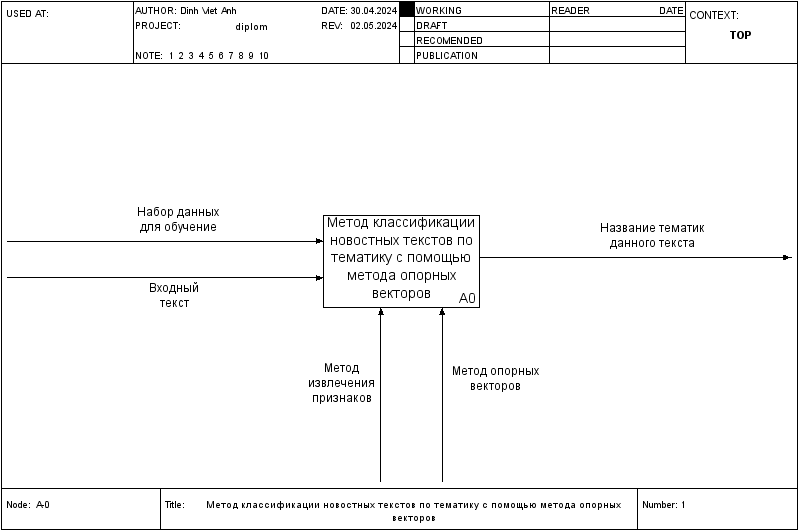
\includegraphics[,scale=0.55]{./img/01_A-0.png}
		\caption{IDEF0-диаграмма нулевого уровня}  
		\label{1-problem}
\end{figure}
\section*{Вывод}
В данном разделе был проведен анализ предметной области. Были рассмотрены методы очистки и предварительной обработки текста. Был проведен обзор методов извлечения признаков из текста. Был рассмотрены и проанализированы основные методы классификации текстов. Была представлена формализованная постановка задачи в виде IDEF0-диаграммы.

В разрабатываемом методе предлагается использовать подход, основанный на использовании TF-IDF для извлечения признаков, для классификации текстов использован метод опорных векторов.